%=======================================================================================================
% Mapping Documentation
%=======================================================================================================
\documentclass[xcolor=rgb,svgnames,dvipsnames]{article}
% \usepackage[bookmarks=true]{hyperref}  % this changes the page location !
\usepackage[bookmarks=true,colorlinks=true,linkcolor=blue]{hyperref}

% \input documentationPageSize.tex
\hbadness=10000 
\sloppy \hfuzz=30pt

% \voffset=-.25truein
% \hoffset=-1.25truein
% \setlength{\textwidth}{7in}      % page width
% \setlength{\textheight}{9.5in}    % page height

\usepackage{calc}
\usepackage[lmargin=.75in,rmargin=.75in,tmargin=.75in,bmargin=.75in]{geometry}

\input homeHenshaw

% \usepackage{epsfig}
\usepackage{graphics}    
\usepackage{moreverb}
\usepackage{amsmath}
% \usepackage{fancybox}  % this destroys the table of contents!
% \usepackage{subfigure}
\usepackage{multicol}

\usepackage{amsmath}
\usepackage{amssymb}
% \input{pstricks}\input{pst-node}
% \input{colours}

\usepackage{tikz}
\input trimFig.tex

% \input{clipFig}
\newcommand{\normalss}{\sffamily}
\newcommand{\largess}{\large\sffamily}


\usepackage{makeidx} % index
\makeindex
\newcommand{\Index}[1]{#1\index{#1}}

\renewcommand\floatpagefraction{1.}
\renewcommand\topfraction{1.}
\renewcommand\bottomfraction{1.}
\renewcommand\textfraction{.0}   
\setcounter{totalnumber}{50}
\setcounter{topnumber}{50}
\setcounter{bottomnumber}{50}


% +++++++++++++++++++++++++++++++++++++++++++++++++++++++++++++++++++++++++++++++++++++++++++++++++++++++++++++
\begin{document}


\input wdhDefinitions

\def\uvd    {{\bf U}}
\def\ud     {{    U}}
\def\pd     {{    P}}
\def\id     {i}
\def\jd     {j}
\def\kap {\sqrt{s+\omega^2}}
% \newcommand{\grad}{\nabla}

\newcommand{\mapping}{\homeHenshaw/Overture/mapping}
\newcommand{\figures}{\homeHenshaw/OvertureFigures}

\vspace{3\baselineskip}
\begin{flushleft}
  {\Large 
   Mappings for Overture  \\ 
   A Description of the Mapping Class  \\
   and Documentation for Many Useful Mappings \\
  }
\vspace{2\baselineskip}
William D. Henshaw      \\         
Centre for Applied Scientific Computing \\
Lawrence Livermore National Laboratory    \\
Livermore, CA, 94551   \\
henshaw@llnl.gov \\
http://www.OvertureFramework.org\\
\vspace{1\baselineskip}
\today \\
\vspace{\baselineskip}
UCRL-MA-132239
% LA-UR-96-3469

\end{flushleft}

\vspace{1\baselineskip}

\begin{abstract}
This document describes the class {\ff Mapping}. The Mapping class is
used to define transformations. These transformations are used within
Overture to define grids and stretching functions and rotations etc.
The base class is called {\ff Mapping}. Particular mappings such as
a sphere or an annulus are defined by deriving a class from the
base class and defining the particular transformation. 
A number of derived Mappings have been written including
\begin{itemize}
 \item  Various Analytical mappings: LineMapping, SquareMapping, CircleMapping, 
        AnnulusMapping, BoxMapping, CylinderMapping, PlaneMapping, QuadraticMapping, SphereMapping
 \item  AirfoilMapping : for creating airfoil related grids and curves (including some NACA airfoils).
 \item  ComposeMapping : for composing two mappings  
 \item  CompositeSurface : a mapping that represents a collection of sub-surfaces.
 \item  CrossSectionMapping : define a surface by cross-sections
 \item  DataPointMapping : mappings defined by data points  
 \item  DepthMapping : create a 3D grid from a 2D grid by adding a variable depth.
 \item  EllipticTransform: smooth a mapping with an elliptic transform.
 \item  FilletMapping: create a fillet or collar grid to join two intersecting surfaces.
 \item  HyperbolicMapping: create volume grids using hyperbolic grid generation (described else-where).
 \item  IntersectionMapping: a mapping that is the intersection between two other mappings, such as
        the curve of intersection between two surfaces.        
 \item  JoinMapping: create a mapping that can join two intersecting mappings.
 \item  LoftedSurfaceMapping: build a lofted surface such as a wing with a tip.
 \item  MatrixMapping : define a matrix transformation by rotations, scaling, shifts etc.  
 \item  MatrixTransform : apply a matrix transformation to another mapping
 \item  NormalMapping : define a new mapping by extending normals
 \item  NurbsMapping : define a mapping by a NURBS, non-uniform rational b-spline.
 \item  OffsetShell : build offset surfaces and an overlapping edge mapping to join them.
 \item  OrthographicTransform : define an orthographic transform
 \item  ReductionMapping : make a new Mapping from the face or edge of another mapping.
 \item  ReorientMapping: used by ReparameterizationTransform to reorder the domain coordinate directions. 
 \item  ReparameterizationTransform : reparameterize a mapping (e.g. remove singularities, or equidistribute
            grid lines by arclength and curvature, or reorder the domain coordinates).
 \item  RestrictionMapping : define a restriction to a sub-rectangle.
 \item  RevolutionMapping : create a surface or volume of revolution
 \item  RocketMapping : create curves related to rocket geometries.
 \item  SmoothedPolygon : for polygons with smoothed corners  
 \item  SplineMapping: define a cubic spline curve.
 \item  StretchMapping : one-dimensional stretching transformations  
 \item  StretchedSquare : stretch grid lines on the unit interval.
 \item  StretchTransform : stretch grid lines along the coordinate directions 
 \item  SweepMapping : Sweep a 2D Mapping along a curve in 3D.
 \item  TFIMapping : define a grid from given boundary curves by transfinite-interpolation (Coon's patch).
 \item  TrimmedMapping : define a trimmed surface in 3D, the surface has portions removed
        from it (``trimmed'').
 \item  UnstructuredMapping : create an unstructured representation for an existing mapping or 
	read in an manipulate and unstructured mesh.
\end{itemize}
All these classes are described in this document.
\end{abstract}



\tableofcontents

\vspace{3\baselineskip}

% \input StretchMapping.tex
% \end{document} 
% *****************************************************************************

\section{Introduction}

The C++ class ``Mapping'' can be used to define the ``mappings''
(transformations) and their properties. For example, each component grid in an
overlapping grid will contain a member function that defines the mapping from
the unit square (or unit cube) onto the domain covered by the grid. This mapping
may in turn be defined in terms of the curves (or surfaces) that form its
boundaries.  Stretching functions as well as rotations and scalings are all
defined by mappings. The source code documentation for the Mapping classes
can be found in Doxygen generated html form on the Overture webpage {\tt www.OvertureFramework.org}. 
This documentation is based on comments embedded within the source code. 

New mappings are defined by derivation from the base class ``Mapping''.
For example, the class ``MatrixMapping'' is a derived class that
defines transformations such as rotations, scalings and translations.

\def\domaind {{domainDimension}}
\def\ranged {{rangeDimension}}
The mapping class can be used to define mapping functions for curves, areas, 
surfaces, volumes etc.:
$$
     f : \Rv^\domaind \rightarrow \Rv^\ranged ~~~~\domaind\le \ranged ~~,~~ 
     \ranged=0,1,2,3
$$
For example a curve in 2D would have $(\domaind,\ranged)=(1,2)$ and a volume
in 3D would have $(\domaind,\ranged)=(3,3)$

\vspace{\baselineskip\noindent}
$\Rv^\domaind$ is called the {\bf domain}\index{domainDimension} of the mapping while
$\Rv^\ranged$ is called the {\bf range}\index{rangeDimension}.

The domain will either be {\bf \Index{parameter space}} (i.e. unit line, unit square,
or unit cube) or {\bf \Index{cartesian space}} (i.e. physical space with
coordinates $(x_1,x_2,x_3)$). Similarly, the range is either parameter
space or cartesian space.


\newcommand{\classMapping}{%
\parbox{4cm}{\normalss%
\begin{center}\largess
Class Mapping
\end{center} 
\begin{flushleft}
{\tt map(r,x,xr)}\\
{\tt inverseMap(x,r,rx)}\\
{\tt update( ... ))}\\
{\tt getBoundaryCondition(...)}\\
{\tt setBoundaryCondition(...)}\\
{\tt etc.}
\end{flushleft}
}}


\begin{figure} \label{fig:MappingClass}
\begin{center}
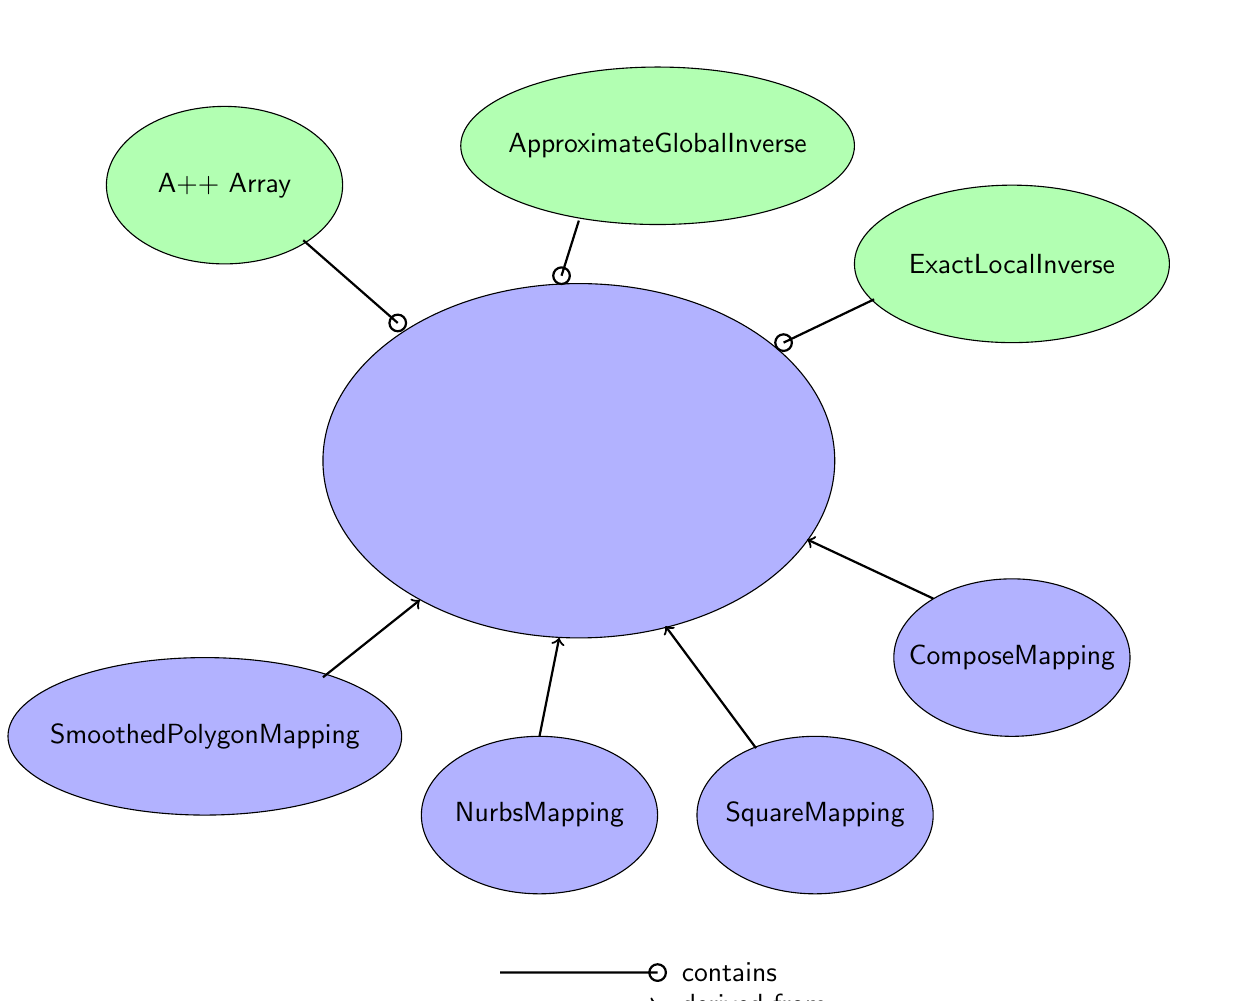
\begin{tikzpicture}
%
\useasboundingbox (-7,-6.5) rectangle (8,5.5);  % set the bounding box (so we have less surrounding white space)
% -- Mapping Class ---
\begin{scope}[xshift=0cm,yshift=0cm]
  \draw[fill=blue!30] (0,0) ellipse(3.25cm and 2.25cm);
  \draw (0,0) node {\classMapping};
\end{scope}
% --- derivation labels
\begin{scope}[xshift=0,yshift=-6.5cm]
  \draw[-,thick] (-1,0) -- (1,0) circle (3pt) node[anchor=west,xshift=5pt] {\normalss contains}; 
  \draw[->,thick] (-1,-.4) -- (1,-.4) node[anchor=west,xshift=5pt]  {\normalss derived from}; 
\end{scope}
% -- A++ --
\begin{scope}[xshift=-4.5cm,yshift=3.5cm]
  \draw[fill=green!30] (0,0) ellipse(1.5cm and 1.cm);
  \draw (0,0) node {\normalss A++ Array};
  \draw[-,thick] (1,-.7) -- (2.2,-1.75) circle (3pt); 
\end{scope}
% -- ApproximateGlobalInverse --
\begin{scope}[xshift=1cm,yshift=4cm]
  \draw[fill=green!30] (0,0) ellipse(2.5cm and 1.cm);
  \draw (0,0) node {\normalss ApproximateGlobalInverse};
  \draw[-,thick] (-1,-.95) -- (-1.22,-1.65) circle (3pt); 
\end{scope}
% -- ExactLocalInverse --
\begin{scope}[xshift=5.5cm,yshift=2.5cm]
  \draw[fill=green!30] (0,0) ellipse(2.cm and 1.cm);
  \draw (0,0) node {\normalss ExactLocalInverse};
  \draw[-,thick] (-1.75,-.45) -- (-2.9,-1.) circle (3pt); 
\end{scope}
% -- SmoothedPolygonMapping --
\begin{scope}[xshift=-4.75cm,yshift=-3.5cm]
  \draw[fill=blue!30] (0,0) ellipse(2.5cm and 1.cm);
  \draw (0,0) node {\normalss SmoothedPolygonMapping};
  \draw[->,thick] (1.5,.75) -- (2.73,1.73); 
\end{scope}
% -- NurbsMapping --
\begin{scope}[xshift=-.5cm,yshift=-4.5cm]
  \draw[fill=blue!30] (0,0) ellipse(1.5cm and 1.cm);
  \draw (0,0) node {\normalss NurbsMapping};
  \draw[->,thick] (0,1) -- (.25,2.25); 
\end{scope}
% -- SquareMapping --
\begin{scope}[xshift=3.0cm,yshift=-4.5cm]
  \draw[fill=blue!30] (0,0) ellipse(1.5cm and 1.cm);
  \draw (0,0) node {\normalss SquareMapping};
  \draw[->,thick] (-.75,.85) -- (-1.9,2.4); 
\end{scope}
% -- ComposeMapping --
\begin{scope}[xshift=5.5cm,yshift=-2.5cm]
  \draw[fill=blue!30] (0,0) ellipse(1.5cm and 1.cm);
  \draw (0,0) node {\normalss ComposeMapping};
  \draw[->,thick] (-1.,.75) -- (-2.6,1.5); 
\end{scope}
%
% draw grid for debugging
% \draw[step=.5cm,gray] (-7,-7) grid (8,5.5);
\end{tikzpicture}
\end{center}
\caption{Diagram for the Mapping Class. A Mapping defines a continuous representation of grids (e.g. annulus or sphere) and more
generally transformations from $\Real^m\rightarrow\Real^n$ (e.g. rotation, body of revolution). } 
\end{figure}


% \subsection{Properties:} 
% 
% There are many properties of interest. Not all properties apply to
% all mapping types. Each mapping can be queried to determine its
% properties.
% 
% \begin{itemize}
%   \item Boundary condition type (true boundary, periodic boundary or
%         interpolation)
%   \item Periodicity (is the mapping or its derivatives periodic)
%   \item Share information (to indicate whether different surface
%         patches belong to the same surface)
% %  \item Invertible (can we invert the mapping?), maybe we should always
% %        define an appropriate inverse (?), for example the inverse of
% %        a curve in 2D could be the closest point. 
%   \item $(\domaind,\ranged)$ dimensions of domain and range
%   \item number of points to use when plotting the mapping, or default
%         number of points to us on the grid
% %  \item Perioidicity of space: is the mapping embedded in a space that
% %        is periodic 
%   \item Coordinate system: cartesian, spherical, cylindrical, polar, 
%         toroidal.      \hfil\break
%         This determines the form of $\partial\xv/\partial\rv$, and will
%         allow us to remove singularities. \hfil\break
%         We will also want to know if the coordinate system is a
%         hemi-sphere $0\le \phi\le \pi/2$, or a sphere cut in half
%         in the other direction $0\le\theta\le\pi$.
%         We may want to define 
%         ``spherical'' plus a range on the coordinates:
%         $\phi_a \le \phi \le \phi_b$, $\theta_a\le \theta \le \theta_b$.
%   \item Other topology information, does the grid have singularities
% \end{itemize}


\vfill\eject
\subsection{Example:}
Here is a simple example of creating and evaluating
a mapping and its inverse. 
(file {\ff example1.C})
{\footnotesize
\listinginput[1]{1}{\mapping/example1.C}
}

%---------------------
\section{Class Mapping}
%---------------------

The base class for mappings is the class {\tt Mapping}.




\subsection{Enum Types }

The following enum types are members of Class Mapping. 

\noindent
Here are the enumerators for the possible spaces for the domain and range
{\footnotesize
\begin{verbatim}
enum mappingSpace{  
                   parameterSpace,    // bounds are [0,1]
                   cartesianSpace }   // default (-infinity,infinity)
                 };
\end{verbatim}
}
\noindent
For example, a stretching function will normally map from {\ff parameterSpace}
to {\ff parameterSpace}. A square grid will usually be a mapping from
{\ff parameterSpace} to {\ff cartesianSpace} (i.e. physical space
with coordinates $(x_1,x_2,x_3)$). A rotation will normally be a mapping from
{\ff cartesian space} to {\ff cartesian space}.

\vspace{\baselineskip\noindent}
Here are the enumerators used to define the \Index{periodicity} of the mapping
(i.e. possible values for {\ff getIsPeriodic})
{\footnotesize
\begin{verbatim}
  enum periodicType
  {
    notPeriodic,
    derivativePeriodic,    // Derivative is periodic but not the function
    functionPeriodic       // Function is periodic
  };
\end{verbatim}
}


\vspace{\baselineskip\noindent}
Here are the enumerators for the \Index{coordinate systems} that we can use for the domain
or the range
{\footnotesize
\begin{verbatim}
enum coordinateSystem{
                       cartesian,                 //  x,y,z
                       spherical,           //  phi/pi, theta/2pi, r
                       cylindrical,         //  theta/2pi, z, r 
                       polar,               //  r, theta/2pi, z
                       toroidal             //  theta1/2pi, theta2/2pi, theta3/2pi
                     };

\end{verbatim}
}
\noindent
Coordinate systems are discussed in greater detail later.

\vspace{\baselineskip\noindent}
Here are the enumerators for the items that we save names for in the
form of character strings,
{\footnotesize
\begin{verbatim}
enum mappingItemName
{
  mappingName,      // mapping name
  domainName,       // domain name
  rangeName,
  domainAxis1Name, // names for coordinate axes in domain
  domainAxis2Name, 
  domainAxis3Name, 
  rangeAxis1Name,  // names for coordinate axes in range
  rangeAxis2Name, 
  rangeAxis3Name 
};
\end{verbatim}
}
\noindent
The names are assigned and retrieved with the the member functions
{\ff setName} and {\ff getName}.


Here are the enumerators used to supply options to {\ff setBasicInverseOption}
{\footnotesize
\begin{verbatim}
  enum basicInverseOptions  // options for basicInverse
  {
    canDoNothing,
    canDetermineOutside,
    canInvert
  };
\end{verbatim}
}
\noindent
Use the {\ff setBasicInverseOption} or {\ff getBasicInverseOption}
functions to retrieve or change these values.


Here are enumerators for the types of Mapping \Index{coordinate systems}, these are
used to optimize the computation of difference approximations to functions
defined on grids derived from this mapping.
{\footnotesize
\begin{verbatim}
  enum mappingCoordinateSystem
  {
    rectangular,               // rectangular mapping
    conformal,                 // conformal              : metric tensor is diagonal and ...
    orthogonal,                // orthogonal mapping     : metric tensor is diagonal
    general                    // general transformation : no special properties
  };
\end{verbatim}
}
\noindent Use the {\ff setMappingCoordinateSystem} and {\ff getMappingCoordinateSystem}
functions to retrieve or change the mapping coordinate system.

% \subsection{Constructors}
% 
% 
% Here is the default constructor with default values:
% 
% \begin{tabbing}
% {\ff MatrixMapping(}\={\ff int m=3,xxxxxxxxxxxxxxxxxxxxxxxxxxx}\= \kill
% {\ff MatrixMapping(}\>{\ff int domainDimension=3,      }\> \\
%               \>{\ff int rangeDimension=3,                           }\\ 
%               \>{\ff mappingSpace domainSpace=parameterSpace,   }\\
%               \>{\ff mappingSpace rangeSpace=cartesianSpace,   }\\
%               \>{\ff coordinateSystem domainCoordinateSystem=cartesian,  }\\
%               \>{\ff coordinateSystem rangeCoordinateSystem=cartesian );}\\
% \end{tabbing}
% 
% 


%% \subsection{Member Functions}
%% In the following {\ff real} will denote either {\ff float} or{\ff double}.

%% \input MappingInclude.tex

\subsubsection{Periodic Mappings}\index{periodic mappings}
  The possible values returned by the function {\ff getIsPeriodic} or passed to
the function {\ff setIsPeriodic} are given by the enumerator {\ff periodicType}:
{\footnotesize
\begin{verbatim}
  enum periodicType
  {
    notPeriodic,
    derivativePeriodic,    // Derivative is periodic but not the function
    functionPeriodic       // Function is periodic
  };
\end{verbatim}
}

\subsection{Member function {\ff map}}

Here is an example of an implementation of the {\ff \Index{map}} member
function. The mapping function is implemented  so that it can evaluate
the mapping for an array of points.
{\footnotesize
\begin{verbatim}

  const int axis1 = 0;
  const int axis2 = 1;

void map( realArray & r, realArray & x, realArray & xr = nullArray, MappingParams & params = nullParams)
{
    Index I = getIndex( r,x,xr,base,bound,computeMap,computeMapDerivative );

    if( computeMap )
    {
      x(I,axis1)=2.*r(I,axis1)+xa; 
      x(I,axis2)=2.*r(I,axis2)+ya;
    }
    if( computeMapDerivative )
    { 
      xr(I,axis1,axis1)=2.;         
      xr(I,axis1,axis2)=0.;  
      xr(I,axis2,axis1)=0.;
      xr(I,axis2,axis2)=2.;
    }
}
\end{verbatim}
}
The function {\ff getIndex} returns an A++ index object that can be used when
evaluating the mapping. Alternatively the variables {\ff base} and {\ff bound}
can be used; note that {\ff I.getBase(axis1)=base} and {I.getBound(axis1)=bound}.
{\ff getIndex} is described later in this section. 

The default
argument for the {\ff xr} array is {\ff nullArray} which is a static 
member function of the Mapping Class. 

The argument {\ff params} is not used in this example. It is used, for example,
to indicate whether the derivatives should be returned in a different coordinate system,
such as sphericalPolar.
The default
argument for {\ff params} is {\ff nullparms} which is a static 
member function of the MappingParams Class.

\subsection{Member function {\ff getIndex }}

The function {\ff \Index{getIndex}} returns an Index object that
can be used for A++ operations. The function {\ff getIndex} also assigns
values to the
variables {\ff base}, {\ff bound}, {\ff computeMap} and
{\ff computeMapDerivative}. Note that {\ff base} and {\ff bound} are
consistent with the base and bound of the Index object returned by
{\ff getIndex}.
The base and bound and Index object
are determined by the first dimension of {\ff r}. For example
if {\ff r} is dimensioned {\ff r(0:9,3)} then {\ff base=0}, and
{\ff bound=9} and {\ff getIndex(...)=Index(base,bound-base+1)}.  
The variable {\ff computeMap} is set to {\ff TRUE}
if dimensions of the array {\ff x} can hold the index object.
The variable {\ff computeMapDerivative} is set to {\ff TRUE}
if dimensions of the array {\ff xr} can hold the index object.

Thus, calling map with a null array (such as {\ff Mapping::nullArray;})
in the place of {\ff x} (or {\ff xr}) will cause the mapping function
not to evaluate {\ff x} (or {\ff xr}).

\subsection{Member functions {\ff \Index{inverseMap}} and {\ff \Index{basicInverse}}}

These member functions evaluate the inverse of the mapping for
an array of points. The derivatives of the inverse mapping can
also be obtained. By default an inverse is defined for
all mappings
whose ${\ff domainDimension} \le {\ff rangeDimension}$. 
This inverse uses Newton's method to invert the mapping.
If the mapping can be inverted more quickly using
another method then you can supply your own inverse.

\begin{itemize}
 \item {\ff inverseMap} : This is the primary function to call
if you want to invert the mapping. This function will call
{\ff basicInverse} if it has been supplied. If the mapping
is a transformation from parameter space to cartesian space
(such as a mapping that defines a grid) then one normally 
should NOT supply this function but instead supply the
{\ff basicInverse} function. The reason for this is that
the {\ff inverseMap} must in general be able to invert
the mapping when space is periodic.
However, if the mapping is a transformation from parameter
space to parameter space (such as a stretching transformation)
or a transformation from cartesian space to cartesian space
(such as a rotation) then one can supply the {\ff inverseMap}
function.

\item {\ff basicInverse} : This routine should be supplied
if the mapping can be inverted quickly and the mapping
is a transformation from parameter space to cartesian space.
The {\ff basicInverse} function does not need to take into 
account the fact that space may be periodic. To indicate that
a {\ff basicInverse} has been supplied you should use
{\ff setBasicInverseOption(canInvert)}. 
\end{itemize}



% The parameter {\ff params} can normally be
% omitted, unless the mapping sits in a periodic space (see section
% ?? for more details).

The {\ff inverseMap} function is automatically defined for all mappings
whose ${\ff domainDimension} \le {\ff rangeDimension}$. 
When ${\ff domainDimension} < {\ff rangeDimension}$ (for example,
a curve in 2D) the inverse is
defined as the closest point in the least squares sense ($L_2$ norm).


If the mapping is a transformation from parameter space to
cartesian space and the mapping can be inverted with an
analytic formula then you should write the {\ff basicInverse} member function.
Here is an example
{\footnotesize
\begin{verbatim}
   const int axis1 = 0;
   const int axis2 = 1;
//==================================================================================
// Here is the basic Inverse (this is an inverse that does not know how
//  to deal with space being periodic)
//=================================================================================
void SquareMapping::basicInverse( const realArray & x, realArray & r, realArray & rx )
{
  Index I = getIndex( x,r,rx,base,bound,computeMap,computeMapDerivative );

  if( computeMap )
  {
    r(I,axis1)=(x(I,axis1)-xa)/(xb-xa); 
    r(I,axis2)=(x(I,axis2)-ya)/(yb-ya); 
  }
  if( computeMapDerivative )
  {
    rx(I,axis1,axis1)=1./(xb-xa);
    rx(I,axis1,axis2)=0.;
    rx(I,axis2,axis1)=0.;
    rx(I,axis2,axis2)=1./(yb-ya);
  }
}
\end{verbatim}
}


If the mapping is a transformation from parameter space to parameter
space or from cartesian space to cartesian space and the mapping 
can be inverted easily then you should write an {\ff inverseMap} function.
Here is an example from the {\ff MatrixMapping} class:
{\footnotesize
\begin{verbatim}
void MatrixMapping::
inverseMap( const realArray & x, realArray & r, realArray & rx, MappingParameters & params )
{ 
  Index I = getIndex( x,r,rx,base,bound,computeMap,computeMapDerivative );

  if( (Mapping::debug/64) % 2 ==1  )
    cout << "MatrixMapping::inverseMap - params.isNull =" << params.isNull << endl;
  
  if( computeMap )
    for( int i=axis1; i<domainDimension; i++ )
    {
      r(I,i)=matrixInverse(i,3);              // holds shift
      for( int j=axis1; j<rangeDimension; j++)
      {
        r(I,i)=r(I,i)+matrixInverse(i,j)*x(I,j);
      }
    }

  if( computeMapDerivative )
    for( int i=axis1; i<domainDimension; i++ )
    {
      for( int j=axis1; j<rangeDimension; j++)
      {
        rx(I,i,j)=matrixInverse(i,j);
      }
    }
\end{verbatim}
}

% Normally one should use the default inverseMap function since this
% will usually be the most efficient way to invert the mapping. There
% are two exceptions. If the mapping can be inverted with an
% analytic formula then you may want to write a new version of inverseMap.
% There is a complication, however. Mappings that will be inverted
% by CMPGRD must know how to deal with the case of space being periodic.
% (The {\ff params} argument will indicate if space is periodic and what
% the periodicity vectors are).
% The second exception is if the mapping is defined as the composition
% of two other mappings. The default inverseMap function will still
% work in this case but it may not be as efficient as possible.
% In this case you should probably use the 
% ``ComposeMapping'' class to define the mapping, or in the event
% that this is not possible, you can
% look at how the inverseMap function is defined by the ``ComposeMapping'' class.


\subsubsection{Member Functions {\ff getName} , {\ff setName} }

These functions get or set the name for any of the items defined in the
enum {\ff mappingItemName}:
\begin{tabbing}
{\ff item =}   \= \kill
{\ff item =}   \>  {\ff mappingClassName } \\
               \>  {\ff mappingName } \\
               \>  {\ff domainName } \\
               \>  {\ff rangeName } \\
               \>  {\ff domainAxis1Name } \\
               \>  {\ff domainAxis2Name } \\
               \>  {\ff domainAxis3Name } \\
               \>  {\ff rangeAxis1Name } \\
               \>  {\ff rangeAxis2Name } \\
               \>  {\ff rangeAxis3Name } \\
\end{tabbing}
These names can be used for plotting labels, for example.
For example
{\footnotesize
\begin{verbatim}

  StretchMapping stretch;                              // create a mapping
  stretch.setName( mappingName, "myStretchMapping" );  // assign the mapping name
  ...
  cout << " Mapping name = " << stretch.getName( Mapping::mappingName ) << endl;

\end{verbatim}
}


\subsection{ Coordinate singularities }\index{coordinate singularity}

The {\ff getTypeOfCoordinateSingularity} function can be used
to determine if a given side of a mapping has a singularity.
The possible types of singularities are 
{\footnotesize
\begin{verbatim}
  enum coordinateSingularity
  {
    noCoordinateSingularity,   //  no coordinate singularity
    polarSingularity           //  grid lines go to a point along the side
  };

\end{verbatim}
}
A {\ff polarSingularity} means that the grids lines converge to a point.
For example, the standard representation for a sphere would have
a {\ff polarSingularity} on the two sides corresponding to 
$\phi=0$ and $\phi=\pi$.

Information about singularities is used by the {\ff inverseMap}.

\subsection{Coordinate systems and coordinateEvaluationType }

Some mappings will have the capability to return
the mapping derivatives in different forms, corresponding to different
\Index{coordinate systems}. Use the {\ff setCoordinateEvaluationType} function to 
indicate that a mapping can return the derivatives in the specified form.
These alternative forms of the derivatives can
be used by a grid generator to remove coordinate singularities.
Here is an example taken from the {\ff SphereMapping} Class:

{\footnotesize
\begin{verbatim}

void SphereMapping::
map( const realArray & r, realArray & x, realArray & xr, MappingParameters & params )
{
  Index I = getIndex( r,x,xr,base,bound,computeMap,computeMapDerivative );

  int i;
  switch (params.coordinateType)
  {
  case cartesian:  // mapping returned in cartesian form

    if( computeMap )
    {
      x(I,axis1)=radius(r(I,axis3))*cos(twoPi*r(I,axis2))*sin(Pi*r(I,axis1))+x0; 
      x(I,axis2)=radius(r(I,axis3))*sin(twoPi*r(I,axis2))*sin(Pi*r(I,axis1))+y0;
      x(I,axis3)=radius(r(I,axis3))*cos(Pi*r(I,axis1))+z0;
    }
    if( computeMapDerivative )
    {
      xr(I,axis1,axis1)=radius(r(I,axis3))*cos(twoPi*r(I,axis2))*Pi*cos(Pi*r(I,axis1)); 
        ...
    }
    
    break;

  case spherical: // Mapping returned in spherical form : (phi,theta,r) 
                  // derivatives: ( d/d(phi), (1/sin(phi))d/d(theta), d/d(r) )

    if( computeMap )
    {
      x(I,axis1)=radius(r(I,axis3))*cos(twoPi*r(I,axis2))*sin(Pi*r(I,axis1))+x0; 
      x(I,axis2)=radius(r(I,axis3))*sin(twoPi*r(I,axis2))*sin(Pi*r(I,axis1))+y0;
      x(I,axis3)=radius(r(I,axis3))*cos(Pi*r(I,axis1))+z0;
    }
    if( computeMapDerivative )
    {
      xr(I,axis1,axis1)=radius(r(I,axis3))*cos(twoPi*r(I,axis2))*Pi*cos(Pi*r(I,axis1)); 
        ...
    }
    break;
  default:
    cerr << "Sphere::map: ERROR not implemented for coordinateType = " 
         << params.coordinateType << endl;
    exit(1);
  }
}
\end{verbatim}
}

\subsection{Class MappingParams}

Additional parameters are passed to the {\ff map} and {\ff inverseMap} functions
by an object of the class {\ff MappingParams}. \index{mapping parameters}

\subsubsection{ Data Members}
\begin{tabbing}
{\ff ApproximateGlobalInverse *approximateGlobalInversexx}xx \= \kill
{\ff int isNull}                     \> True if parameters have not been set    \\
{\ff int periodicityOfSpace}         \> =0,1,2,3                                \\
{\ff realArray periodicityVector}    \> vector(s) for periodicity               \\
{\ff MappingWorkSpace workSpace}     \> work space                              \\
{\ff int computeGlobalInverse}       \> TRUE by default                         \\
{\ff coordinateSystem coordinateType}\> evaluate mapping in this coordinate system \\
{\ff ApproximateGlobalInverse *approximateGlobalInverse} \> pointer \\
{\ff ExactLocalInverse *exactLocalInverse} \> pointer \\
\end{tabbing}
If space is periodic, then the parameters {\ff periodicityOfSpace} and
{\ff periodicityVector} must be set in calls to {\ff inverseMap}. 
Here is an example:

{\footnotesize
\begin{verbatim}

#include "Mapping.h"
#include "Square.h"

void main()
{

  realArray r1(10,2), x1(10,2), xr1(10,2,2);
  realArray r2(10,2), x2(10,2), rx2(10,2,2);

  SquareMapping square();

  MappingParameters periodicParams;
  // here is where we set the periodicity of Space, this should be consistent
  // with the periodicity of ALL mappings
  periodicParams.periodicityOfSpace=1;
  periodicParams.periodicityVector(axis1,axis1)=2.; // set vector to (2,0)
  periodicParams.periodicityVector(axis2,axis1)=0.;

  cout << "=============Periodic in Space=============" << endl;
  cout << " ---Call square map with an array of values:" << endl;
  for( i=0; i<10; i++ )
  {
    r1(i,axis1)=i/9.; 
    r1(i,axis2)=i/9.; 
  }
  square.map( r1,x1,xr1 );  // get x1 and xr1 at an array of points
  for( i=0; i<10; i++ )
    printf(" Square: r= (%6.3f,%6.3f) x = (%7.4f,%7.4f)\n",
      r1(i,axis1),r1(i,axis2),x1(i,axis1),x1(i,axis2));

  cout << " ---Call square inverseMap with an array of values:" << endl;
  for( i=0; i<10; i++ )
  {
    x2(i,axis1)=1.5*x1(i,axis1); 
    x2(i,axis2)=x1(i,axis2); 
  }
  r2=1.;  // initial guess
  square.inverseMap( x2,r2,rx2,periodicParams );  
  for( i=0; i<10; i++ )
    printf(" Square: x= (%6.3f,%6.3f) r = (%7.4f,%7.4f)\n",
      x2(i,axis1),x2(i,axis2),r2(i,axis1),r2(i,axis2));

}
\end{verbatim}
}



The {\ff inverseMap} member function of the {\ff ComposeMapping} class will
use the {\ff computeGlobalInverse} parameter.

\subsection{Class ApproximateGlobalInverse}

This class is used to define an \Index{inverse!approximate global inverse} of a mapping.
The approximate global inverse computes an approximate inverse to the
mapping. This approximate inverse should be good enough so that a
Newton iteration will converge.

Each mapping contains a pointer to an ApproximateGlobalInverse, called
{\ff approximateGlobalInverse}. 
This ApproximateGlobalInverse is used by the {\ff inverseMap} member function.

We now describe the default implementation for the ApproximateGlobalInverse.
The default approximate global inverse has a discrete grid that contains
values of the mapping. The inverse finds the closest point on this grid.
The number of points on the grid can be set by the Mapping
member function {\ff setGridDimensions}
or the actual grid to be used can be specified with the ApproximateGlobalInverse
member function {\ff setGrid}. 


%% \input ApproximateGlobalInverseInclude.tex

\subsection{Class ExactLocalInverse}\index{inverse!exact local inverse}

This class defines an exact inverse for a mapping, given a good initial guess.

Each mapping contains a pointer to an ExactLocalInverse, called
{\ff exactLocalInverse}.
This ExactLocalInverse is used by the {\ff inverseMap} member function.

The default ExactLocalInverse uses the Newton algorithm to invert the
mapping (if the mapping is invertible) or uses Newton to find the
closest point ($L_2$-norm) between a point and a surface or curve.


\input inverse.tex

%% \input ExactLocalInverseInclude.tex

\subsection{Registering Mappings and Reading Generic Mappings from the DataBase}
\index{registering a new mapping}

In this section we describe how a mapping can be read from a database file
and contructed even when the function constructing the mapping does not
know the (derived) class to which the mapping belongs. For example, this
situtaion occurs when a container class holds a pointer to a Mapping. The
pointer is of type {\ff Mapping*} but the pointer may point to a derived
class such as {\ff SquareMapping}.  Suppose the container class is saved to a 
database file with the function {\ff Container::put}. When it is read 
back in again with {\ff Container::get} the {\ff get} function will not 
know how to ``get'' the mapping.

To solve this problem each mapping class has a member function {\ff make}
(a virtual member function of the base class) that look likes

{\footnotesize
\begin{verbatim}

Mapping *SquareMapping::make( const String & mappingClassName )
{ // Make a new mapping if the mappingClassName is the name of this Class
  Mapping *retval=0;
  if( mappingClassName==className )
    retval = new SquareMapping();
  return retval;
}
\end{verbatim}
}

The function {\ff make} creates a new mapping of it's own class provided
that the String passed to {\ff make} is the name of it's class.

The Mapping Class contains a static member that is a list of pointers
to Mappings, {\ff mappingList}. Each member of the list points
to an instance of a different derived mapping Class. All possible 
Mapping Class's that may be read from the database should have a
member in {\ff mappingList}.
Here, for example, is how to add members to the {\ff mappingList}:
{\footnotesize
\begin{verbatim}
  CircleMapping circle;
  StretchMapping stretch;
  ...
  Mapping::mappingList.add( &circle );
  Mapping::mappingList.add( &stretch );
\end{verbatim}
}

The {\ff makeMapping} member function of the Mapping Class can be used
to make a Mapping corresponding to a given class name. 
The {\ff makeMapping} function takes as input the name of a class
that it should try to make. For example, the argument to {\ff makeMapping}
may be the String {\ff className=="SquareMapping"}. The {\ff makeMapping} function
goes through it's list of mappings,
calling the {\ff make} member function of each mapping, until
it finds the mapping class that is able to make a {\ff "SquareMapping"}. 

{\footnotesize
\begin{verbatim}

//================================================================
//  Get a mapping from the database
//    This routine looks through the list of mapping Class's
//    that have been placed on the mappingList and tries to
//    find one that knows how to make a mapping whose name
//    is equal to the input argument className
// 
//  Input:
//    const String & className 
//       : name of the mapping class to get from the database file
//    Dir dir
//       : directory on the database where the mapping is stored
//    const String & name
//       : the database name for the mapping
//
//================================================================
Mapping* Mapping::makeMapping( const String & className )
{ //  Try to construct a mapping 
    Mapping *retval = 0;
    for( Item *ptr=mappingList.start; ptr; ptr=ptr->next )
      if( retval = ptr->val->make( className ) ) break;
    return retval;
}
\end{verbatim}
}


Here is the definition of a container class that calls {\ff makeMapping}
in order to construct a mapping. The container class has a pointer
to a generic Mapping. There is no trouble saving the mapping to
a database with the {\ff put} member function. However when it 
reads the mapping back from the database it must be able to
construct an instance of the appropriate derived class; this is
done by {\ff makeMapping}. {\bf Note} that we assume that each Mapping
class has a data member {\ff String className} that holds the name
of the class.
{\footnotesize
\begin{verbatim}
class Container
{ 
public:
  Mapping *mapPointer;

  ...

  void get( const Dir & dir, const String & name )
   {
     // Make a new directory unless name="."
     Dir subDir = name=="." ? dir : dir.findDir(name);

     // Look for the className of the Mapping:
     Dir mappingDir = subDir.findDir("containedMapping");
     String mappingClassName;
     mappingDir.get( mappingClassName,"className" );

     // Make an instance of the appropriate derived Mapping class
     mapPointer = Mapping::makeMapping( mappingClassName );
     getMap=TRUE;
     mapPointer->get( subDir,"containedMapping" );   // get the mapping

   }
  void put( const Dir & dir, const String & name )
   {  
     // destory the directory if it exists
     if( !dir.locateDir(name).isNull() )
       dir.destroy(name, " R");
     Dir subDir = name=="." ? dir : dir.createDir(name);

     mapPointer->put( subDir,"containedMapping" );  // save the mapping

   }

};

\end{verbatim}
}


%\subsubsection{Bounds}
%
%The arrays of type {\ff Bound}, such as
% {\ff domainBound} and  {\ff rangeBound} hold the bounds
%for each side of each axis, {\ff domainBound[axis][side]}.
%The value of {\ff side} is $0$ or $1$ corresponding to the lower
%and upper bounds. The value of {\ff axis} is one of $0,1,2$.
%
%A bound can be a real number, an integer or a fraction f=n/d. 
%(The Bound class is described later in this document).
%The bounds can be assigned with the {\ff set} member function:
%{\footnotesize
%\begin{verbatim}
%      domainBound[axis][side].set( 1. );    // set bound to be a real number
%      domainBound[axis][side].set( 1  );    // set bound to be an integer
%      domainBound[axis][side].set( 1,2 );   // set bound to be a fraction, 1/2
%\end{verbatim}
%}
%In this way
%the bounds can be specified precisely, bounds specified as
%integers, {\ff [0,1]} are more than those specific by real
%numbers {\ff [0.,1.]}. In addition we may specify bounds
%as plus or minus infinity by the fractions $0/-1$ and $0/1$.


\clearpage
\input AnnulusMapping.tex


\clearpage
\input AirfoilMapping.tex

\clearpage
\input BoxMapping.tex

\clearpage
\input CircleMapping.tex

\clearpage
\input ComposeMapping.tex

\clearpage
\input CompositeSurface.tex

\clearpage
\input CrossSectionMapping.tex


\clearpage  % new page plus draw figures
\input CylinderMapping.tex

\clearpage
\input DataPointMapping.tex

\clearpage
\input DepthMapping.tex


\clearpage
\input EllipticTransform.tex

\clearpage
\input FilletMapping.tex

\clearpage
\subsection{HyperbolicMapping}

See the separate document {\sl The Overture Hyperbolic Grid Generator} \cite{HyperbolicGuide}.
% \input HyperbolicMapping.tex
% \clearpage


\input IntersectionMapping.tex
\clearpage
\input JoinMapping.tex
\clearpage
\input LineMapping.tex
\clearpage
\input LoftedSurfaceMapping.tex


\clearpage
\input MatrixMapping.tex

\clearpage
\input MatrixTransform.tex
\clearpage
\input NormalMapping.tex
\clearpage
\input NurbsMapping.tex
\clearpage
\input OffsetShell.tex
\clearpage
\input OrthographicTransform.tex
\clearpage
\input PlaneMapping.tex
\clearpage
\input QuadraticMapping.tex
\clearpage
\input ReductionMapping.tex
\clearpage
\input ReorientMapping.tex
\clearpage
\input ReparameterizationTransform.tex
\clearpage
\input RestrictionMapping.tex
\clearpage
\input RevolutionMapping.tex
\clearpage
\input RocketMapping.tex
\clearpage
\input SmoothedPolygon.tex
\clearpage
\input SphereMapping.tex
\clearpage
\input SplineMapping.tex

\clearpage
\input SquareMapping.tex
\clearpage
\input StretchMapping.tex
\clearpage
\input StretchedSquare.tex
\clearpage
\input StretchTransform.tex

\clearpage
\input SweepMapping.tex

\clearpage
\input TFIMapping.tex
\clearpage
\input TrimmedMapping.tex
\clearpage
\input UnstructuredMapping.tex
\clearpage

% \section{Utility Classes: Fraction, Bound, Triangle}

% ------ utility classes ---------

\input Fraction.tex

\section{Class Triangle}\index{triangle}

The {\tt Triangle} class is used to represent a triangle in three dimensional space.
It has a function for determining how two triangles intersect that is used by the 
{\tt IntersectionMapping} class.

%% \input TriangleInclude.tex

\clearpage
\bibliography{\homeHenshaw/papers/henshawPapers,\homeHenshaw/papers/henshaw}
\bibliographystyle{siam}

\printindex

\end{document}








